% !TeX root = main.tex
\documentclass[english]{report}
\usepackage[usenames,dvipsnames]{color} 
\usepackage[utf8]{inputenc}
\usepackage{amsmath}
\usepackage{mathtools}
\usepackage[margin=1.5cm]{geometry}
\usepackage{float}
\usepackage{listings}
\usepackage{hyperref}
\usepackage{amssymb}
\usepackage{enumerate}
\usepackage[shortlabels]{enumitem}
\usepackage{subcaption}
\usepackage{titlesec}
\usepackage{xr}
\usepackage{graphicx}
\usepackage[demo]{rotating}
\usepackage{wrapfig}
\usepackage{ragged2e}
\usepackage{multicol}
\usepackage{textcomp, gensymb}
\usepackage[useregional]{datetime2}[showzone=false]
\RequirePackage{xkeyval}
\RequirePackage{etoolbox}
\usepackage{csvsimple, booktabs, siunitx}
\usepackage[titletoc]{appendix}

% Custom configurations and commands
% !TeX root = ..\main.tex
% Custom Commands
\newcommand\dif{\mathop{}\!\mathrm{d}} %dx for integrals \dif{x}
\newcommand\var[1]{\text{Var}\left[\,#1\,\right]} %Var[]
\newcommand\cov[2]{\text{Cov}\left[\,#1,#2\,\right]} %Cov[x1,x2]
\newcommand\E[1]{\text{E}\left[\,#1\,\right]} %E[]
\newcommand\IQR{\text{I}\text{Q}\text{R}}
\newcommand\nline{\par\vspace{4pt}}
\newcommand\sOneSize{0.4625}
\newcommand\sTwoRes{0.70}
\newcommand\PgSz{\scriptsize}
%% Defaults for LstListing Environment
\lstset{
  caption=\lstname,
  basicstyle=\scriptsize\ttfamily, % the size of the fonts that are used for the code
  numbers=left,                   % where to put the line-numbers
  numberstyle=\tiny\color{black},  % the style that is used for the line-numbers
  stepnumber=1,                   % the step between two line-numbers. If it is 1, each line
                                  % will be numbered
  numbersep=5pt,                  % how far the line-numbers are from the code
  backgroundcolor=\color{white},  % choose the background color. You must add \usepackage{color}
  showspaces=false,               % show spaces adding particular underscores
  showstringspaces=false,         % underline spaces within strings
  showtabs=false,                 % show tabs within strings adding particular underscores
  frame=single,                   % adds a frame around the code
  rulecolor=\color{black},        % if not set, the frame-color may be changed on line-breaks within not-black text (e.g. commens (green here))
  tabsize=2,                      % sets default tabsize to 2 spaces
  captionpos=t,                   % sets the caption-position to top
  breaklines=true,                % sets automatic line breaking
  breakatwhitespace=false,        % sets if automatic breaks should only happen at whitespace
  }
%% Defining Style for R Code and Python within LstListing Environment
% !TeX root = ..\main.tex
\lstdefinestyle{R}{ 
  language=R,                     % the language of the code
  keywordstyle=\color{RoyalBlue},      % keyword style
  commentstyle=\color{YellowGreen},   % comment style
  stringstyle=\color{ForestGreen}      % string literal style
}

\lstdefinelanguage{PythonPlus}[]{Python}{
  morekeywords=[1]{,as,assert,nonlocal,with,yield,self,True,False,None,} % Python builtin
  morekeywords=[2]{,__init__,__add__,__mul__,__div__,__sub__,__call__,__getitem__,__setitem__,__eq__,__ne__,__nonzero__,__rmul__,__radd__,__repr__,__str__,__get__,__truediv__,__pow__,__name__,__future__,__all__,}, % magic methods
  morekeywords=[3]{,object,type,isinstance,copy,deepcopy,zip,enumerate,reversed,list,set,len,dict,tuple,range,xrange,append,execfile,real,imag,reduce,str,repr,}, % common functions
  morekeywords=[4]{,Exception,NameError,IndexError,SyntaxError,TypeError,ValueError,OverflowError,ZeroDivisionError,}, % errors
  morekeywords=[5]{,ode,fsolve,sqrt,exp,sin,cos,arctan,arctan2,arccos,pi, array,norm,solve,dot,arange,isscalar,max,sum,flatten,shape,reshape,find,any,all,abs,plot,linspace,legend,quad,polyval,polyfit,hstack,concatenate,vstack,column_stack,empty,zeros,ones,rand,vander,grid,pcolor,eig,eigs,eigvals,svd,qr,tan,det,logspace,roll,min,mean,cumsum,cumprod,diff,vectorize,lstsq,cla,eye,xlabel,ylabel,squeeze,}, % numpy / math
}

\lstdefinelanguage{PyBrIM}[]{PythonPlus}{
  emph={d,E,a,Fc28,Fy,Fu,D,des,supplier,Material,Rectangle,PyElmt},
}

\lstdefinestyle{colored}{ %
  basicstyle=\ttfamily,
  backgroundcolor=\color{white},
  commentstyle=\color{green}\itshape,
  keywordstyle=\color{blue}\bfseries\itshape,
  stringstyle=\color{red},
}

\definecolor{darkred}{rgb}{0.6,0.0,0.0}
\definecolor{darkgreen}{rgb}{0,0.50,0}
\definecolor{lightblue}{rgb}{0.0,0.42,0.91}
\definecolor{orange}{rgb}{0.99,0.48,0.13}
\definecolor{grass}{rgb}{0.18,0.80,0.18}
\definecolor{pink}{rgb}{0.97,0.15,0.45}

\lstdefinestyle{colorEX}{
  basicstyle=\ttfamily,
  backgroundcolor=\color{white},
  commentstyle=\color{darkgreen}\slshape,
  keywordstyle=\color{blue}\bfseries\itshape,
  keywordstyle=[2]\color{blue}\bfseries,
  keywordstyle=[3]\color{grass},
  keywordstyle=[4]\color{red},
  keywordstyle=[5]\color{orange},
  stringstyle=\color{darkred},
  emphstyle=\color{pink}\underbar,
}
%% Hyperlink customization
\hypersetup{
  %hidelinks    = false, %Remove color box
  frenchlinks  = false, %Small caps for hyperlinks
  colorlinks   = true, %Colours links instead of boxes
  urlcolor     = blue, %Colour for external hyperlinks
  linkcolor    = black, %Colour of internal links
  citecolor   = black   %Colour of citations
}
%% Extra spacing on matrices
\makeatletter
\renewcommand*\env@matrix[1][\arraystretch]{%
  \edef\arraystretch{#1}%
  \hskip -\arraycolsep
  \let\@ifnextchar\new@ifnextchar
  \array{*\c@MaxMatrixCols c}}
\makeatother
%%Capitalising \autoref
\renewcommand*{\chapterautorefname}{Chapter}
\renewcommand*{\subsectionautorefname}{Subsection}
\renewcommand*{\sectionautorefname}{Section}
%%Merging list of tables and figures
\def\table{\def\figurename{Table}\figure}
\let\endtable\endfigure 
\renewcommand\listfigurename{List of Figures and Tables}
%%Formating Chapter spacing and linebreak
\titleformat{\chapter}[hang] 
{\normalfont\huge\bfseries}{\chaptertitlename\ \thechapter:}{1em}{}
\titlespacing*{\chapter}{0pt}{0pt}{5pt}
\begin{document}
\pagenumbering{roman} %Start roman numbering
% !TeX root = ..\main.tex
\begin{titlepage}
	\centering
	% 
\includegraphics[width=0.35\textwidth]{Title/logo.eps} \par
	
\includegraphics[width=0.35\textwidth]{Title/logo.png} \par
	%{\scshape\LARGE Exeter University \par}
	\vspace{0.25cm}
	{\scshape\Large MTHM005 - Mathematical Sciences Project\par}
	\vspace{0.5cm}
	{\huge\bfseries Pricing Asian Options\par}
    \vspace{0.10cm}
	{\Large Candidate Number: 145670}
	\vspace{0.2cm}
	\flushleft
	Supervised by	Prof.~\textsc{Byott} \hfill	{\large \today\par}
    \par
    \centering
	{\large \textbf{Abstract}}
	\par
    
Options are contracts that grant the right, but not the obligation to buy or sell an underlying asset at a set price on a specified date.
    
    %Insert some cool abstract that makes our examiner go, "hmm that's a pretty good abstract".

    \vfill
    All documents and \textsc{Matlab} files available here: \par \small{\url{https://github.com/leele2/Mathematics-in-Business-Project}}
\end{titlepage}
\begingroup %Disable page break between TOC and LOFAT
    \let\clearpage\relax          
    \renewcommand{\baselinestretch}{1.0} %Set spacing for TOC
    \tableofcontents
    \vspace{0.4cm}
    \listoffigures
\endgroup
% !TeX root = ..\..\main.tex
\chapter{Introduction}
\pagenumbering{arabic} %Start roman numbering

This report studies a vital financial derivative in today's markets, namely options. The importance of the option market has been shown by empirical studies which suggest that option trading improves information efficiency in the broader stock market \cite{PanInfoEffic,li2021effect}, and also that firms with listed options experience lower implied cost of equity capital \cite{naikerLowEquity}; indicating that options trading reduces the cost of capital \cite{li2021effect}. The popularity of the options market can easily be seen by the exponential growth in their trading volume since standardized, exchange-traded stock options were first listed in The Chicago Board Options Exchange in 1973 \cite{markham2002financial}; shown in \autoref{C1fig:OptionVolume}. In 2020 single stock option trading volume became higher than the underlying stock volume for the first time ever \cite{yahooOptions}. 
\nline
It is this explosive popularity and significance which have motivated this report. We will begin by describing standard options and explore popular methods that are used to price them. We will then move onto Asian options and look at the literature surrounding how to price them before implementing several pricing methods with the use of \textsc{Matlab}. Furthermore, we will then take an analytical approach to determine how Asian options can be priced accurately and efficiently.

\begin{figure}[H]
    \centering
    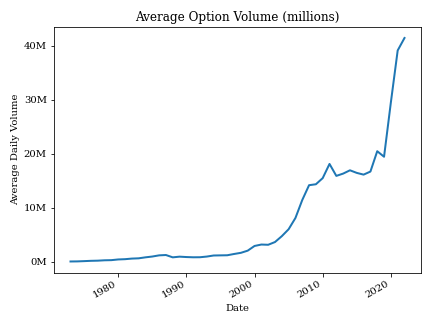
\includegraphics[width=0.65\textwidth]{Chapters/C1/plots/OptionVolume.png}
    \caption{Time series plot of the average daily option and future contracts trading volume per annum. Data provided by the Options Clearing Corporation (OCC) \cite{THEOCC}. 
    Source code: \autoref{ApPy:lst option volume plot}
    }
    \label{C1fig:OptionVolume}
\end{figure}

\section{A brief overview of call and put options}

Options are a particular type of financial derivative, a contract that details the conditions under which payments are made between two counterparties. They are purchased for a set fee, and in return the buyer is granted the right, but not the obligation to buy or sell an underlying asset - such as commodities, stocks or bonds - for a predetermined price (the strike price) on or before a determined date (the expiry date).
\nline
Call options allow the buyer to purchase an asset for the strike price at a future date. The buyer can make a return if the value of the asset is worth more than the strike price when exercised. Alternatively, put options allow the buyer to sell an asset for the strike price at a future date and the buyer can make a return if the value of the asset is worth less than the strike price when exercised.
\nline
The option market is widely considered a venue for informed trading \cite{li2021effect,hu2014,chak2004}, that is, investors trading with superior knowledge of the probability distribution of share prices, through either access to private information or skillful processing of public information \cite{grossman1975application}. 

\subsection{A short history of option trading}

The history of financial options can be traced as far back as 6th century b.c. when ancient Greek mathematician and philosopher Thales of Miletus predicted through his astrological knowledge there was going to be a great olive harvest. As he did not have much money, he used what he had as a deposit on the rights to the local olive presses; due to no competition he secured this at a relatively low price. When the harvest proved to be bountiful leading to high demand, Thales charged a high price for use of the presses and reaped a considerable profit. His deposit gave him the right but not the obligation to hire the presses, thus his losses were limited to his initial deposit \cite{OptionFirst, 1877aristotle}.
\nline
Whilst this is quite a positive look on option trading, throughout history this has not always been the case. During the Dutch tulip bubble of the seventeenth century when the popularity of tulips as status symbols drove up their price, creating a bubble \cite{dash2011tulipomania}. Tulip growers would buy puts to protect their profits in case the price of tulip bulbs went down and wholesalers would buy calls to protect against the risk of tulip bulbs going up. When the bubble eventually burst, due to the unregulated nature of the option market, there was no way to force investors to fulfil their obligations of the options contracts. This ultimately led to options gaining a dubious reputation and bans were later placed on them within Britain between 1733-1860 \cite{OptionBan}. 
\nline
During the late nineteenth century, brokers started to arrange deals between buyers and sellers of options for particular stocks at prices that were arranged between the two parties. Trades were arranged similarly until the 1960s when the options market started to become regulated by the Chicago Board of Trade. In 1973, the Chicago Board of Options Exchange (CBOE) began trading and for the first time options contracts were properly standardized. At the same time, the Options Clearing Corporation was established for centralized clearing and ensuring the proper fulfillment of contracts, ensuring that they were honored \cite{markham2002financial}.

%There also exist other types of financial derivatives, such as futures contracts - these are similar to options except that they carry the obligation to buy or sell the particular asset - and the first implementation of such derivatives dates back to as early as ancient Greece. For example, during this time period, farmers benefited from opportunities to sell corn within agricultural markets under futures contracts (or known more simply as futures). It is likewise thought that, within a contracted transaction, Aristotle provided the rights to use olive presses to fellow ancient Greek philosopher Thales of Miletus. This resulted in profit for the investor, who had astutely speculated an overly abundant harvest. 

%On the other hand, the first example of options came during the Middle Ages, when traders developed contracts that granted the buyer with the right to purchase the cargo of a ship on arrival. Options were likewise used during the infamous Dutch tulip bubble of the seventeenth century, where contracted prices for the newly fashionable tulip bulbs skyrocketed for a period of months, before eventually collapsing. The first organised options market was created within London during the same century.

%This being said, options were often traded in fairly dubious circumstances, with parties not fulfilling their obligations leading to big losses for investors. Within the USA, this can be seen mainly as a result of the unstandardised options markets that existed during the late nineteenth century. Accordingly, at the turn of the century Louis Bachelier published a thesis detailing a method to model option prices, incorporating both Brownian motion and the Wiener process. This greatly influenced the eventual publication of the Black-Scholes formula, as discussed below within Section $\ref{sec:personnel}$.

\subsection{Standard options}

A standard option comes in two styles; European: which restricts the holder of the option to only exercise the option on the expiry date, and American: which allows the holder to exercise the option at anytime up till or on the expiry date. They will take the current value of the underlying asset as the spot price - that is the price that the asset can be purchased for on the open market. The payoff in this case then becomes the difference between the spot price and strike price.

\subsection{Asian options}

Whilst standard options involve using the spot price as the underlying value of the asset; this is not always the case with so-called exotic options. Exotic options differ in their payment structures, expiration dates, and/or strike prices. In the case of exotic fixed-strike price Asian options, the averaging price of the asset is used in place of the underlying asset value. This differs from fixed-price Asian options which instead use the averaging price of the asset to take place of the strike price. These are the two main variations of Asian style options but both of these can be varied further in how the averaging is calculated, for example: geometrically, arithmetically, average taken every day or average taken at the start of each month and so on. They can be varied further by having an expiry structure matching a European or American style option.

\section{Pricing options}

Since the holder of the contract is not obliged to exercise the contract at the expiry time, they do not hold any liability in the absence of a price to purchase the option. The problem then becomes, what is the correct price to charge the holder of the option to balance this inequality of liability.

\subsection{Pricing standard options}

\subsubsection{Binomial method}

\subsubsection{Black-Scholes Formula}

\subsection{Pricing Asian options}

\subsubsection{Hull-White model}

\subsubsection{Costabile adjusted binomial method}

\subsubsection{Analytical solution for geometric average Asian options}

% \begingroup
% \RaggedRight
\bibliographystyle{alpha}
\bibliography{mybibliography.bib}
% \endgroup
\pagebreak
% !TeX root = ..\main.tex
\begin{appendices}
    \chapter{\textsc{Matlab} Files}
        All files can be found: \small{\url{https://github.com/leele2/Mathematics-in-Business-Project/tree/master/MATLAB%20Files}}
\end{appendices}

\end{document}